\documentclass[journal]{IEEEtran} % `journal` option per ITherm conference template
\IEEEoverridecommandlockouts
% Needed only to identify funding in the first footnote. Comment out if unneeded.
\usepackage{cite}
\usepackage{amsmath,amssymb,amsfonts}
\usepackage{algorithmic}
\usepackage{graphicx}
\usepackage{textcomp}
\usepackage{xcolor}
\usepackage{booktabs}
\usepackage{tabularx}
\usepackage{url}
\usepackage{tikz}
\usetikzlibrary{arrows.meta,positioning,shapes.geometric,decorations.pathreplacing,calc}

\def\BibTeX{{\rm B\kern-.05em{\sc i\kern-.025em b}\kern-.08em
    T\kern-.1667em\lower.7ex\hbox{E}\kern-.125emX}}
\begin{document}

\title{Symbolic Formal Verification of Quantum Circuits for Post-Quantum
Cryptography Governance in Critical Infrastructures}

\author{%
    \IEEEauthorblockN{1\textsuperscript{st} Rafael Silvestrim}%
    , \IEEEauthorblockN{2\textsuperscript{nd} Manoel F. Amaral Filho}%
    , \IEEEauthorblockN{3\textsuperscript{rd} Alberjan Pinto}%
    , \IEEEauthorblockN{4\textsuperscript{th} Juan J. Gouvea}%
    , \IEEEauthorblockN{5\textsuperscript{th} Iury V. de Bessa}%
    , \IEEEauthorblockN{6\textsuperscript{th} Anderson F. P. dos Santos}%
    , \IEEEauthorblockN{7\textsuperscript{th} Lucas C. Cordeiro}%
    \\%
    \IEEEauthorblockA{\textit{Post Graduate Program in Electrical Engineering, Federal University of Amazonas, Manaus, Brazil}}\\
    \IEEEauthorblockA{\textit{International Center of Software Technology (CITS.AM), Manaus, Brazil}}\\
    \IEEEauthorblockA{\textit{Juno Woz Labs, Manaus, Brazil}}\\
    \IEEEauthorblockA{\textit{Department of Electricity, Federal University of Amazonas, Manaus, Brazil}}\\
    \IEEEauthorblockA{\textit{Military Institute of Engineering (IME), Rio de Janeiro, Brazil}}\\
    \IEEEauthorblockA{\textit{Department of Computer Science, University of Manchester (UoM), Manchester, UK}}\\
    \IEEEauthorblockA{rafael.silvestrim@ufam.edu.br · manoel.amaral@ufam.edu.br · alberjan.pinto@cits.br · junogouvea@gmail.com · iury.bessa@ufam.edu.br · anderson.santos@ime.eb.br · lucas.cordeiro@manchester.ac.uk}
}

\maketitle

\begin{abstract}
The migration to post-quantum cryptography (PQC) in critical infrastructures demands not only the replacement of
classical algorithms but also the rigorous validation of quantum artifacts employed in auxiliary migration processes prior to execution on real hardware. This paper proposes and demonstrates a symbolic formal verification pipeline based on the ESBMC-Q\# engine, a Verify
Before Execution (VBE) strategy. The pipeline transpiles Q\# programs into symbolic C representations, under both an IEEE 754 encoding and an exact rational encoding over $\mathbb{Z}[\omega]$, injects assertions for physical
unitarity, functional equivalence, and logical fidelity, and exhaustively explores the state space up to bound $k$ via Bounded Quantum
Model Checking (BQMC). The evaluation covers Clifford circuits, a non-Clifford $T$-gate sequence, and a PQC-supporting quantum random number generator; deliberate fault injection demonstrates detection of a phase-flip violation that sampling-based tests miss, and a scalability benchmark reports where SMT solving degrades under symbolic initial states. Each verdict becomes a digitally signed JSON-LD evidence record, mapped to an IM-PQC governance decision by a CI/CD gate. The work targets TRL 4 in the dual-use (civil/defense) context, contributing to digital sovereignty.
\end{abstract}

\begin{IEEEkeywords}
Post-quantum cryptography · Quantum formal verification · ESBMC-Q\# · Bounded Quantum Model Checking · Technology governance · Critical infrastructures · Dual-use · Digital sovereignty
\end{IEEEkeywords}

\section{Introduction}
The emergence of quantum computers capable of breaking public-key cryptography (RSA, ECC) has motivated global standardization efforts. In August 2024, NIST published the first PQC standards: ML-KEM (FIPS 203), ML-DSA (FIPS 204), and SLH-DSA (FIPS 205) \cite{ref1,ref2,ref3}. The NSA CNSA 2.0 establishes migration deadlines for national security systems between 2025 and 2033 \cite{ref4}, and NIST IR 8547 defines depreciation schedules for RSA and ECC for federal use \cite{ref5}. The ``Store Now, Decrypt Later'' (SNDL) threat renders the protection of military facilities, C2 systems, and power grids particularly critical, given their long lifecycles and inherent vulnerability windows \cite{ref6}.

The PQC algorithms standardized by NIST (ML-KEM, ML-DSA, SLH-DSA) are classical algorithms designed to resist quantum attacks; they are not implemented by quantum circuits. The circuits addressed in this work are therefore not PQC implementations but \textit{quantum validation artifacts} employed in auxiliary processes of the PQC migration---quantum random number generation, key distribution, hybrid-computing subroutines---whose correctness must be established before execution on real hardware. Instance-based testing verifies only finite subsets of the state space, which is insufficient for high-criticality quantum circuits \cite{ref7}. Symbolic formal verification via Bounded Model Checking (BMC) exhaustively explores the transition space up to a limit $k$, generating mathematical evidence and formal counterexamples. The ESBMC-Q\# engine extends the ESBMC verifier, widely validated for C/C++ programs \cite{ref8,ref9,ref10}, to quantum programs in Q\#. Recent contributions on the verification of secure architectures (Arm CCA \cite{ref12}) and on integrating LLMs with ESBMC for formal specification \cite{ref13} provide direct foundations for the proposed pipeline.

Table~\ref{tab:trl} summarizes the research stage and TRL evolution.

% Table I: research stage / TRL
\begin{table}[!t]
\centering
\caption{Note on Research Stage and TRL Evolution}
\label{tab:trl}
\footnotesize
\begin{tabularx}{\columnwidth}{@{}lX@{}}
\toprule
\textbf{Category} & \textbf{Description} \\
\midrule
Current TRL & \textbf{TRL 3 -- TRL 4}: analytical and experimental proof of critical functions completed; integrated pipeline validated in a laboratory environment. \\
Validation & Complete VBE loop: Clifford, non-Clifford ($T$) and QRNG artifacts verified; deliberate fault blocked; signed evidence records; GHZ-$n$ scalability benchmark. \\
Target & \textbf{TRL 5}: multi-qubit non-Clifford artifacts and validation in operationally relevant environments (Section~\ref{sec:roadmap}). \\
\bottomrule
\end{tabularx}
\end{table}

\textbf{Research Question}: How to ensure, prior to execution on real quantum hardware, that quantum artifacts employed in the PQC transition preserve physical and logical properties, with auditable formal evidence for the governance of critical infrastructures? \textbf{Hypotheses}: H1: Symbolic verification detects violations that sample testing does not identify; H2: BQMC reduces operational risk and experimental cost; H3: Formal evidence integrates into PQC governance frameworks.
\textbf{Contributions (C1--C5)}:
(C1) Pre-execution VBE pipeline for Q\# in a PQC context;
(C2) ESBMC-Q\# as an auditable evidence mechanism;
(C3) Integration of formal verification $\leftrightarrow$ IM-PQC governance;
(C4) Experimental demonstration with fault injection, non-Clifford and QRNG artifacts, and a scalability benchmark;
(C5) Dual-use and digital sovereignty framework.

\section{Related Work}

Do and Ogata \cite{ref14} propose symbolic model checking via Maude with LTL for quantum protocols. Bauer-Marquart et al. \cite{ref7} introduce symQV, the first automatic symbolic verification tool for quantum programs, while Chen et al. \cite{ref15} develop AutoQ 2.0 based on automata. Xu et al. \cite{ref16} conduct a systematic review of formal verification for PQC, identifying the gap in governance integration that this work occupies. Within the ESBMC ecosystem, Cordeiro et al. \cite{ref8,ref9,ref10} consolidated the SMT-based verifier, with recent extensions including Python \cite{ref11}, Kotlin \cite{ref17}, Solidity \cite{ref18}, and the verification of Arm security components \cite{ref12}.

The tradition of formal verification in critical systems within the PPGEE/UFAM group is established by Bessa and Cordeiro through DSVerifier \cite{ref19,ref20}, focused on embedded digital controllers for UAVs, and extended by Silvestrim and Cordeiro \cite{ref24} to resource-constrained embedded platforms, establishing a methodology for hardware-software co-verification that this work carries into the quantum domain. In terms of governance, Hasan et al. \cite{ref21} and Alnahawi et al. \cite{ref22} address migration frameworks and protocol transitions, yet fall short of generating auditable formal evidence---the gap that our ESBMC-Q\# pipeline fills by bridging formal software verification with the requirements of the PQC transition in critical infrastructures.

\section{Formal Verification Model}
The formal verification of quantum circuits is modeled as a Bounded Model Checking (BMC) problem over a quantum transition system. The verification tuple is defined as:

\begin{equation}
    P = \langle \Sigma, \Sigma_0, T, \Phi \rangle
\end{equation}

\noindent where:
\begin{itemize}
    \item $\Sigma$: is the set of symbolic states (vectors in the Hilbert space represented symbolically);
    \item $\Sigma_0 \subseteq \Sigma$: represents the set of initial states;
    \item $T : \Sigma \rightarrow \Sigma$: is the transition function, where each logic gate is treated as a symbolic unitary transformation;
    \item $\Phi$: is the property (\textit{assertion}) to be verified.
\end{itemize}

ESBMC-Q\# utilizes an SMT \textit{solver} (Z3, Boolector) to decide whether $\exists$ a symbolic assignment such that $\Phi$ is violated in the expression $\Phi \wedge Translation(Program, k)$. An \textbf{UNSAT} result implies the correctness of the circuit up to the limit $k$, while a \textbf{SAT} result generates an auditable formal counterexample. Unlike sampling-based tests, which verify heuristically chosen cases, symbolic verification explores all trajectories up to the bound $k$, producing mathematical rather than probabilistic evidence. Fig.~\ref{fig:model} illustrates the explored state space: from $\sigma_0 \in \Sigma_0$, each gate is applied as a symbolic transition $T$ up to the bound $k$, where $\Phi$ is decided as SAT or UNSAT.

% Figure 1: model P = <Sigma, Sigma0, T, Phi>
\begin{figure}[!t]
\centering
\resizebox{\columnwidth}{!}{%
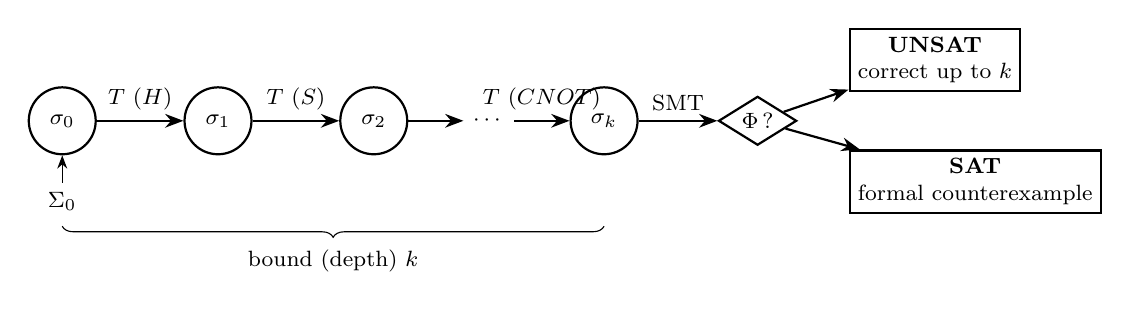
\begin{tikzpicture}[>=Stealth, font=\footnotesize,
    state/.style={circle, draw, thick, minimum size=8.5mm, inner sep=1pt},
    dec/.style={diamond, draw, thick, aspect=1.6, inner sep=1.5pt, align=center},
    res/.style={rectangle, draw, thick, align=center, inner sep=3pt}]
    \node[state] (s0) {$\sigma_0$};
    \node[state, right=11mm of s0] (s1) {$\sigma_1$};
    \node[state, right=11mm of s1] (s2) {$\sigma_2$};
    \node[right=7mm of s2] (dots) {$\cdots$};
    \node[state, right=7mm of dots] (sk) {$\sigma_k$};
    \node[dec, right=10mm of sk] (phi) {$\Phi$\,?};
    \node[res, above right=2mm and 9mm of phi] (unsat) {\textbf{UNSAT}\\correct up to $k$};
    \node[res, below right=2mm and 9mm of phi] (sat) {\textbf{SAT}\\formal counterexample};
    \draw[->, thick] (s0) -- node[above]{$T$ ($H$)} (s1);
    \draw[->, thick] (s1) -- node[above]{$T$ ($S$)} (s2);
    \draw[->, thick] (s2) -- (dots);
    \draw[->, thick] (dots) -- node[above]{$T$ ($CNOT$)} (sk);
    \draw[->, thick] (sk) -- node[above]{SMT} (phi);
    \draw[->, thick] (phi) -- (unsat);
    \draw[->, thick] (phi) -- (sat);
    \node[below=3.5mm of s0] (sig0) {$\Sigma_0$};
    \draw[->] (sig0) -- (s0);
    \draw[decorate, decoration={brace, mirror, amplitude=4pt}]
        ($(s0.south)+(0,-9mm)$) -- ($(sk.south)+(0,-9mm)$)
        node[midway, below=5pt]{bound (depth) $k$};
\end{tikzpicture}}
\caption{Symbolic verification model $P = \langle \Sigma, \Sigma_0, T, \Phi \rangle$: gate-induced transitions explored up to depth $k$, with SAT/UNSAT decision point.}
\label{fig:model}
\end{figure}

\section{VBE Pipeline Architecture}
The formal verification of quantum circuits is structured into a four-stage pipeline, designated as the \textit{Verify Before Execution} (VBE) flow, illustrated in Fig.~\ref{fig:pipeline}.

\begin{itemize}
    \item \textbf{Stage E1: Q\# Programming.} The developer implements the quantum circuit using Microsoft's Q\# language, leveraging native support for Clifford+$T$ gates ($X, H, S, T, CNOT$) and measurements.
    \item \textbf{Stage E2: Symbolic Transpilation (qsharp2c.py).} A Python-based transpiler converts the Q\# source into a C harness, where each gate is represented as a symbolic linear operation over amplitudes. The transpiler implements two amplitude encodings: (i) \textit{exact rational arithmetic} over the ring $\mathbb{Z}[\omega]/\sqrt{2}^{\,k}$, $\omega = e^{i\pi/4}$, the standard exact representation for Clifford+$T$ amplitudes \cite{ref26}: amplitudes are integer 4-tuples with a shared denominator exponent, and all gate actions and property checks are integer-only (zero tolerance); and (ii) \textit{IEEE 754 floating point}, enabled in ESBMC via \texttt{--floatbv}, which models the concrete numerical behavior of amplitudes and enables the verification of stability invariants such as norm preservation ($|\alpha|^2 + |\beta|^2 = 1$) under rounding. Encoding (ii) is the default, so that the verified model reflects the arithmetic actually executed by classical control software; encoding (i) is applied to purely algebraic properties (unitarity and functional equivalence of Clifford+$T$ operators), for which an \textbf{UNSAT} verdict constitutes an exact algebraic proof. Section~\ref{sec:results} reports experiments under both. Assertions for unitarity ($U^\dagger U = I$), functional equivalence, and logical fidelity are automatically injected, selected per artifact by source-level directives.
    \item \textbf{Stage E3: ESBMC-Q\#.} The C harness is processed by the ESBMC-Q\# engine, which performs Bounded Quantum Model Checking (BQMC) with a bound $k = \text{circuit length} + 1$, exploring all symbolic paths via SMT solvers.
    \item \textbf{Stage E4: IM-PQC Evidence.} The engine returns \textbf{UNSAT}, \textbf{SAT}, or \textbf{TIMEOUT}. Each verdict is serialized as a JSON-LD evidence record, digitally signed (Ed25519), and integrated into the IM-PQC governance framework, following the verdict-to-decision mapping detailed in Section~\ref{sec:governance}.
\end{itemize}

% Figure 2: VBE pipeline
\begin{figure}[!t]
\centering
\resizebox{\columnwidth}{!}{%
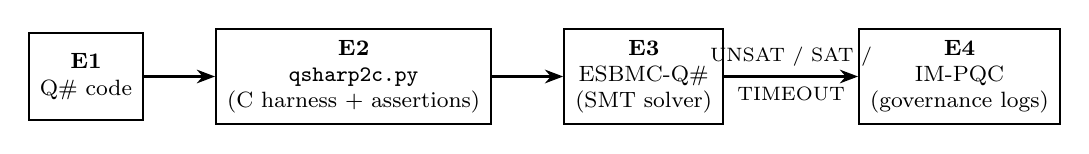
\begin{tikzpicture}[>=Stealth, font=\footnotesize, node distance=9mm,
    stage/.style={rectangle, draw, thick, align=center, inner sep=4pt, minimum height=11mm}]
    \node[stage] (e1) {\textbf{E1}\\Q\# code};
    \node[stage, right=of e1] (e2) {\textbf{E2}\\\texttt{qsharp2c.py}\\(C harness + assertions)};
    \node[stage, right=of e2] (e3) {\textbf{E3}\\ESBMC-Q\#\\(SMT solver)};
    \node[stage, right=17mm of e3] (e4) {\textbf{E4}\\IM-PQC\\(governance logs)};
    \draw[->, thick] (e1) -- (e2);
    \draw[->, thick] (e2) -- (e3);
    \draw[->, thick] (e3) -- node[above]{\scriptsize UNSAT / SAT /} node[below]{\scriptsize TIMEOUT} (e4);
\end{tikzpicture}}
\caption{VBE pipeline architecture in 4 stages: from Q\# source to auditable governance logs.}
\label{fig:pipeline}
\end{figure}

\section{Verified Properties}
Table~\ref{tab:properties} consolidates the verified properties, their operational definitions, and relevance to PQC security and governance.

% Table II: formal properties
\begin{table}[!t]
\centering
\caption{Formal Properties for PQC Circuit Validation}
\label{tab:properties}
\footnotesize
\begin{tabularx}{\columnwidth}{@{}l>{\raggedright\arraybackslash}X>{\raggedright\arraybackslash}X>{\raggedright\arraybackslash}X@{}}
\toprule
\textbf{Property} & \textbf{Operational Definition} & \textbf{PQC Relevance} & \textbf{Governance Role} \\
\midrule
Unitarity & $U^\dagger U = I$ & Physical consistency & Compliance \\
Equivalence & $State_{out} = State_{ref}$ & Logic validation & Accountability \\
Fidelity & $|\langle \psi | \phi \rangle|^2 \approx 1$ & Noise resilience & Risk mgmt. \\
Uniformity & $P(0) = P(1) = 1/2$ & QRNG unbiasedness & Auditability \\
\bottomrule
\end{tabularx}
\end{table}

\section{Experimental Methodology}
Five circuit categories were selected to test hypotheses H1--H3:
\begin{itemize}
    \item \textbf{Q1: Identity Circuits.} $X \cdot X$ and $H \cdot H$ (1 qubit); $CNOT \cdot CNOT$ (2 qubits).
    \item \textbf{Q2: Entanglement.} Bell-state preparation ($H$, $CNOT$), asserting the target amplitudes of $(|00\rangle + |11\rangle)/\sqrt{2}$.
    \item \textbf{Q3: Deliberate Failure.} $S$ applied twice on $|1\rangle$ where identity was asserted ($S^2 = Z \neq I$), as a negative control for H1.
    \item \textbf{Q4: PQC-Supporting Artifacts.} (a) a QRNG for key-material generation, asserting outcome uniformity $P(0) = P(1) = 1/2$ before measurement; and (b) the non-Clifford sequence $H \cdot T \cdot T$, asserting equivalence with $H \cdot S$ ($T^2 = S$), verified under both encodings.
    \item \textbf{Q5: Scalability Set.} GHZ-$n$ circuits ($H$ followed by a $CNOT$ chain) with increasing $n$ and bounds $k \in \{n, 2n\}$, used exclusively for the benchmark of Section~\ref{sec:benchmark}.
\end{itemize}

\textbf{Hardware and Environment Settings}: All verification experiments were executed on an Apple M5 machine (macOS, 32 GB RAM), using ESBMC v8.4.0 (64-bit arm64) with the Z3 v4.16.0 SMT solver. The IEEE 754 encoding enables the \texttt{--floatbv} theory, mapping continuous amplitudes to genuine floating-point semantics, including rounding; the exact encoding uses pure integer arithmetic and requires no tolerance.

\textbf{Experimental Protocol}: For each circuit: (1) Q\# source implementation; (2) transpilation to a C harness via \texttt{qsharp2c.py}, injecting the property assertions; (3) exhaustive state-space exploration via ESBMC-Q\# with bound $k = \text{depth} + 1$; and (4) classification of the result as \textbf{UNSAT} (verified), \textbf{SAT} (counterexample found), or \textbf{TIMEOUT}, followed by the emission of a signed evidence record (Section~\ref{sec:governance}). The C model was cross-validated against an independent state-vector simulator, which recomputes every expected state from the gate matrices and additionally checks the $\mathbb{Z}[\omega]$ ring operations against complex arithmetic; all checks pass. Metrics include verification conditions (VCCs), solver and total runtime, circuit depth, and property validity.

\section{Experimental Results}
\label{sec:results}
\subsection{Experiments 1--3: Functional Correctness and Numerical Stability}
The proposed methodology was evaluated through formal verification of fundamental quantum gates and the generation of an entangled state. Experiments 1 ($X \cdot X$) and 2a ($H \cdot H$) were successfully verified as identities: ESBMC-Q\# generated 4 VCCs for each, solved by Z3 in under 2\,ms, confirming functional equivalence (\textbf{UNSAT}). Furthermore, by encoding the physical invariant of the qubit's norm ($|\alpha|^2 + |\beta|^2 = 1$) via the \texttt{check\_stability} function, the solver proved that the state transitions maintained numerical stability within IEEE 754 floating-point boundaries.

Experiment 2b ($CNOT \cdot CNOT$) and Experiment 3 (Bell state) were verified in the $C^4$ Hilbert space. The $CNOT$ composition was proven to be the identity, and the Bell-state fidelity was confirmed through assertions on the target amplitudes of the entangled state. All experiments returned \textbf{UNSAT} in under 0.4\,s of total engine time. Table~\ref{tab:results} summarizes the performance data.

\subsection{Experiment 4: Deliberate Failure (Central Result)}
To validate the tool's error detection capability, we performed Experiment 4 ($S \cdot S$ on the state $|1\rangle$). Mathematically, $S^2 = Z$, which introduces a phase flip ($-|1\rangle$). By asserting that the final state should be $|1\rangle$, we induced a logic violation. ESBMC-Q\# returned \textbf{SAT} in under 0.2\,s, generating a counterexample that explicitly names the divergent amplitude: the assertion \emph{``functional equivalence: beta ($|1\rangle$) amplitude diverges''} is violated, exposing the phase $-1$ on $|1\rangle$. This confirms the tool's sensitivity to phase-related errors, which are notoriously difficult to detect via conventional statistical sampling (where phase information is collapsed or obscured by measurement).

\subsection{Experiments 5--6: PQC-Supporting and Non-Clifford Artifacts}
Experiment 5 verifies a QRNG artifact, the canonical quantum-native component of PQC key-generation workflows: the uniformity property $P(0) = P(1) = 1/2$ was proven (\textbf{UNSAT}) for the pre-measurement state. Experiment 6 verifies the non-Clifford sequence $H \cdot T \cdot T$ against the reference $H \cdot S$: under IEEE 754 the equivalence holds within the stated tolerance (6a); under the exact $\mathbb{Z}[\omega]$ encoding it is proven as an exact algebraic identity (6b), together with exact unitarity after every gate. While this 1-qubit instance is still classically simulable, it exercises precisely the gate set ($T$) that takes circuits outside the Gottesman--Knill regime.

% Table III: experimental results
\begin{table}[!t]
\centering
\caption{Summary of Experimental Results}
\label{tab:results}
\footnotesize
\setlength{\tabcolsep}{3.0pt}
\begin{tabular}{@{}llllllll@{}}
\toprule
\textbf{Exp.} & \textbf{Circuit} & \textbf{Property} & \textbf{Enc.} & \textbf{$k$} & \textbf{VCCs} & \textbf{Result} & \textbf{Time} \\
\midrule
1  & $X \cdot X$        & Identity    & F & 3 & 4 & UNSAT & 0.32s \\
2a & $H \cdot H$        & Identity    & F & 3 & 4 & UNSAT & 0.18s \\
2b & $CNOT \cdot CNOT$  & Identity    & F & 3 & 3 & UNSAT & 0.18s \\
3  & Bell state         & Fidelity    & F & 3 & 3 & UNSAT & 0.18s \\
4  & $S^2 \neq I$       & Identity    & F & 3 & 5 & \textbf{SAT} & 0.18s \\
5  & QRNG ($H$)         & Uniformity  & F & 2 & 2 & UNSAT & 0.18s \\
6a & $H T T = H S$      & Equivalence & F & 4 & 4 & UNSAT & 0.18s \\
6b & $H T T = H S$      & Equivalence & E & 4 & 6 & UNSAT & 0.13s \\
\bottomrule
\end{tabular}

\vspace{2pt}
\raggedright\scriptsize Enc.: F = IEEE 754 (\texttt{--floatbv}), E = exact $\mathbb{Z}[\omega]$. Z3 decision time $\leq 5$\,ms in all runs.
\end{table}

\subsection{Scalability Benchmark}
\label{sec:benchmark}
To characterize how the approach scales, GHZ-$n$ preparation circuits were verified for increasing qubit counts $n$ (state space $2^n$) and two bounds per $n$, under four regimes of increasing symbolic generality: \emph{func} (concrete initial state $|0\ldots0\rangle$, asserting the target GHZ amplitudes, $k = n$ gates); \emph{basis} (symbolic basis state $|idx\rangle$, $idx < 2^n$ nondeterministic, GHZ followed by its inverse, asserting equivalence, $k = 2n$: one verification covering all $2^n$ basis inputs); \emph{unit} (fully symbolic amplitudes of unit norm, asserting norm preservation, $k = n$); and \emph{ident} (fully symbolic amplitudes, GHZ plus inverse, asserting equivalence, $k = 2n$). Table~\ref{tab:benchmark} reports the results (timeout 300\,s; each sweep stops at its first timeout).

% Table IV: scalability benchmark
\begin{table}[!t]
\centering
\caption{Scalability Benchmark (GHZ-$n$, timeout 300\,s)}
\label{tab:benchmark}
\footnotesize
\setlength{\tabcolsep}{4.5pt}
\begin{tabular}{@{}llrrll@{}}
\toprule
\textbf{Regime} & \textbf{Initial state} & \textbf{$n$} & \textbf{$k$} & \textbf{Verdict} & \textbf{Wall} \\
\midrule
func  & concrete $|0\ldots0\rangle$ & 2  & 2  & UNSAT & 0.12s \\
func  &                             & 4  & 4  & UNSAT & 0.14s \\
func  &                             & 6  & 6  & UNSAT & 0.27s \\
func  &                             & 8  & 8  & UNSAT & 1.53s \\
func  &                             & 10 & 10 & UNSAT & 23.1s \\
func  &                             & 12 & 12 & T/O   & $>$300s \\
\midrule
basis & all $2^n$ basis states      & 2  & 4  & UNSAT & 12.0s \\
basis &                             & 4  & 8  & T/O   & $>$300s \\
\midrule
unit  & all states (norm 1)         & 1  & 1  & T/O   & $>$300s \\
ident & all states (norm 1)         & 1  & 2  & T/O   & $>$300s \\
\bottomrule
\end{tabular}
\end{table}

Three explicit findings emerge. First, with concrete inputs the pipeline scales comfortably to $n = 10$ ($2^{10}$ amplitudes, 23\,s), with cost dominated by symbolic execution rather than solving, and exhausts the budget at $n = 12$. Second, quantifying over all basis inputs simultaneously is feasible at $n = 2$ (12\,s for a single verification covering all four basis inputs) but exceeds the budget at $n = 4$. Third, and most importantly, the fully symbolic regimes exceed the budget already at $n = 1$: deciding quadratic norm constraints over IEEE 754 semantics is the bottleneck of the floating-point theory itself, independent of qubit count. We report this openly: the continuous-symbolic regime is where the exponential nature of BQMC manifests, and pushing this frontier (bit-precise FP solvers, exact-encoding equivalence at scale, abstraction) is the core technical challenge of the roadmap.

\section{Comparison with Conventional Testing}
Table~\ref{tab:comparison} compares the VBE approach with conventional testing, supporting H1 in high-criticality quantum deployments.

% Table V: conventional testing vs VBE
\begin{table}[!t]
\centering
\caption{Comparison between Conventional Testing and VBE Approach}
\label{tab:comparison}
\footnotesize
\begin{tabularx}{\columnwidth}{@{}l>{\raggedright\arraybackslash}X>{\raggedright\arraybackslash}X@{}}
\toprule
\textbf{Feature} & \textbf{Conventional Testing (Sampling)} & \textbf{VBE Approach (Formal Verification)} \\
\midrule
Coverage & Partial (statistical sampling) & Exhaustive (up to bound $k$) \\
Evidence & Probabilistic (shots/counts) & Mathematical (SMT-based proof) \\
Error detection & High-probability states only & Corner cases and rare violations \\
Governance & Limited auditability & Full accountability (JSON-LD logs) \\
Cost & High (real hardware execution) & Low (pre-execution simulation) \\
\bottomrule
\end{tabularx}
\end{table}

\section{Threats to Validity and Soundness}
\label{sec:threats}
\subsection{Soundness of the Transpilation}
Every verdict produced by ESBMC-Q\# is relative to the C model generated by \texttt{qsharp2c.py}. If the transpilation does not faithfully preserve Q\# semantics, an \textbf{UNSAT} result certifies only the C harness, not the original quantum program. Two mitigations are currently in place: (i) each gate is encoded as a fixed, manually reviewed linear transformation over amplitudes, following the formal semantics of $\lambda$-Q\#; and (ii) all circuits were cross-validated against an independent state-vector simulator (distributed with the artifact), which recomputes every expected state from the gate matrices and additionally validates the $\mathbb{Z}[\omega]$ ring operations against complex arithmetic. Cross-validation is itself sampling-based evidence; a by-construction soundness argument relating the generated C semantics to $\lambda$-Q\# remains future work and is a precondition for trusting UNSAT verdicts on larger circuits.

\subsection{The Gottesman--Knill Caveat}
Most circuits verified here belong to the Clifford group, which, by the Gottesman--Knill theorem, is efficiently simulable on classical computers. Experiment 6 shows that the pipeline is not restricted to stabilizer semantics: the non-Clifford $T$ gate is verified under both encodings, including an exact algebraic proof. Still, every instance evaluated here remains classically simulable at its scale. The value demonstrated at this stage is exhaustive symbolic coverage up to the bound $k$ (quantifying over all input states, which simulation cannot do), machine-checkable counterexamples, and auditable evidence generation. The decisive test requires multi-qubit non-Clifford circuits (Toffoli, $T$ over $n \geq 2$ qubits), where classical simulation becomes intractable; this extension is scheduled in the roadmap (Section~\ref{sec:roadmap}).

\subsection{Bounded Guarantees}
An \textbf{UNSAT} verdict certifies correctness only up to the bound $k$. For the fixed-depth, loop-free circuits considered here, $k = \text{depth} + 1$ makes the verification complete for the stated properties; parametrized or iterative programs will require completeness arguments such as $k$-induction, already supported by ESBMC \cite{ref8}.

\subsection{Numerical Encoding}
The IEEE 754 encoding introduces rounding: violations smaller than the assertion tolerance could be masked, and rounding itself could, in principle, produce spurious counterexamples. Three mitigations apply: assertions use explicit tolerances; the norm-preservation invariant is checked at every transition; and, in the symbolic benchmark, the assumption band on input norms is strictly tighter than the assertion band, so accumulated rounding cannot manufacture a counterexample. The exact $\mathbb{Z}[\omega]$ encoding eliminates this threat class entirely for algebraic properties, as demonstrated in Experiment 6b, where equivalence and unitarity are proven with zero tolerance.

\subsection{External Validity}
The eight runs in Table~\ref{tab:results} form a proof of concept, and Table~\ref{tab:benchmark} bounds what may be extrapolated from them; no scalability claim is made beyond it, and extending the symbolic-input frontier is the central technical objective of the roadmap.

\section{Impact on IM-PQC Governance}
\label{sec:governance}
\subsection{From Verdicts to Governance Decisions}
Each verdict produced by the pipeline has a defined role in the IM-PQC decision process: \textbf{UNSAT} authorizes the promotion of the artifact to the next lifecycle stage and is archived as positive evidence; \textbf{SAT} blocks the artifact at the CI/CD gate, and the formal counterexample is attached to the risk register for correction and re-verification; \textbf{TIMEOUT} triggers escalation to manual review, with an increase of the bound $k$ or decomposition of the circuit. The mapping is implemented: the gate exposes the decision as its process exit code (0 = promote, 1 = block, 2 = escalate), directly enforceable by any CI/CD system. The loop was exercised end-to-end on a PQC-supporting artifact (the QRNG of Experiment 5, promoted with signed evidence) and on a faulty artifact (Experiment 4, blocked with its counterexample archived).

\subsection{Accountability Registry}
Each verification generates a digitally signed (Ed25519, RFC 8032) JSON-LD record containing the circuit ID, pipeline and solver versions, encoding, property, bound $k$, verdict, metrics, and timestamp, providing auditable proof that the artifact was validated (or blocked) prior to any operational use (supporting \textbf{H3}). Fig.~\ref{fig:jsonld} reproduces the actual signed record of Experiment 4, capturing the \textbf{SAT} verdict and the counterexample for the risk register; signatures are verifiable offline with the registry's public key. These records can be attached to security reports and audits, demonstrating compliance with \textbf{NIST SP 800-53} \cite{ref23} and equivalent national standards.

% Figure: JSON-LD evidence record for Experiment 4 (real signed record;
% hex values truncated for presentation)
\begin{figure}[!t]
\centering
\scriptsize
\begin{verbatim}
{
 "@context": "https://w3id.org/security/v2",
 "@type": "VerificationRecord",
 "circuit_id": "TestSIdentity",
 "pipeline": { "transpiler": "qsharp2c.py v2.0",
   "verifier": "ESBMC 8.4.0", "solver": "Z3 4.16.0",
   "flags": "--unwind 1 --z3 --floatbv" },
 "property": "identity",
 "amplitude_encoding": "float",
 "qubits": 1, "circuit_depth": 2, "bound_k": 3,
 "verdict": "SAT",
 "governance_decision": "BLOCK",
 "metrics": { "vccs": 5, "solver_time_s": 0.003 },
 "timestamp": "2026-07-08T05:16:58+00:00",
 "counterexample": "functional equivalence:
                    beta (|1>) amplitude diverges",
 "proof": {
   "type": "Ed25519Signature2020",
   "publicKeyHex": "730c8f6f...6efd7a8b",
   "signatureHex": "e1222034...7e912800" }
}
\end{verbatim}
\caption{Signed JSON-LD evidence record from Stage E4 for Experiment 4 (SAT $\rightarrow$ BLOCK); hex values truncated, metrics abridged.}
\label{fig:jsonld}
\end{figure}

\subsection{Pre-Execution Technology Gate}
The pipeline integrates into \textbf{CI/CD} workflows (GitLab CI, Jenkins) through the gate's exit-code contract, automatically blocking non-compliant circuits before execution on real hardware, as demonstrated by the \textbf{SAT} record of Fig.~\ref{fig:jsonld}, which halts the promotion of the faulty circuit. This is particularly relevant in defense environments, where executing unverified code could compromise sensitive experiments or \textbf{C2 systems}.

\subsection{Dual-Use and Digital Sovereignty}
The same techniques protecting civilian infrastructures (power grids, telecommunications) apply to military systems (C2, tactical cryptography). Research by Prof. Santos on the cybersecurity of \textbf{IEC 61850} critical infrastructures \cite{ref25} directly contextualizes this dual-use dimension. The capability to audit circuits locally, without reliance on foreign solutions, constitutes an essential component of \textbf{technological sovereignty}.

\section{Roadmap and Next Steps}
\label{sec:roadmap}
This work consolidates the analytical and experimental proof of critical functions characteristic of \textbf{TRL 3} and validates the integrated VBE pipeline in a laboratory environment (\textbf{TRL 4}): all four stages were exercised end-to-end, including the signed evidence chain and the blocking gate. The roadmap:

\begin{itemize}
    \item \textbf{2026--2027 (TRL 5):} Multi-qubit non-Clifford circuits (Toffoli, $T$ over $n \geq 2$ qubits), beyond the Gottesman--Knill limitation; exact $\mathbb{Z}[\omega]$ encoding for multi-qubit systems; pushing the symbolic-input frontier (bit-precise FP solvers, abstraction, $k$-induction \cite{ref8}); a formal transpilation soundness argument; and open-source release with full CI/CD automation.
    \item \textbf{2027--2028 (TRL 6):} Validation in a real defense scenario with the Brazilian Army and Navy cryptography laboratories (IME/UFAM partnership); integration with critical system acquisition processes; and submission to regulatory bodies (\textit{e.g.}, INMETRO, ABNT).
\end{itemize}

\section{Conclusion}
This paper presented a VBE symbolic formal verification pipeline for quantum circuits, based on ESBMC-Q\#, with a focus on the PQC transition in critical infrastructures. The verified circuits are validation artifacts of the migration process, not PQC implementations, and include a PQC-supporting QRNG and a non-Clifford $T$ sequence proven equivalent with zero tolerance under the exact $\mathbb{Z}[\omega]$ encoding. The central result (Experiment 4, in which the verifier detected and blocked a phase-flip failure invisible to sample testing) validates \textbf{H1}; the scalability benchmark delimits openly where the symbolic regime meets its exponential cost, and the signed evidence chain closes the loop between verification verdicts and IM-PQC decisions (\textbf{H3}). The primary gap filled is the absence of an operational integration between quantum formal verification and IM-PQC governance with auditable evidence; this work implements and validates that integration in a laboratory environment, within broader doctoral research at PPGEE/UFAM. As next steps, we envision: (1) multi-qubit non-Clifford circuits (Toffoli) beyond the reach of classical simulation; (2) extending the symbolic-input frontier identified in the benchmark; (3) a formal soundness argument for the \texttt{qsharp2c.py} transpilation; (4) CI/CD integration in defense environments; and (5) validation in a real operational scenario.

\section*{Acknowledgments}
The authors thank PPGEE/UFAM, CITS.AM, INDT, IME, Venturus, and the University of Manchester for their support.

\begin{thebibliography}{00}

\bibitem{ref1} National Institute of Standards and Technology (NIST), “Module-Lattice-Based Key-Encapsulation Mechanism Standard,” FIPS 203, Aug. 2024, doi: 10.6028/NIST.FIPS.203.

\bibitem{ref2} National Institute of Standards and Technology (NIST), “Module-Lattice-Based Digital Signature Standard,” FIPS 204, Aug. 2024, doi: 10.6028/NIST.FIPS.204.

\bibitem{ref3} National Institute of Standards and Technology (NIST), “Stateless Hash-Based Digital Signature Standard,” FIPS 205, Aug. 2024, doi: 10.6028/NIST.FIPS.205.

\bibitem{ref4} National Security Agency (NSA), “Commercial National Security Algorithm Suite 2.0,” Cybersecurity Information Sheet, Fort Meade, MD, USA, Sep. 2022.

\bibitem{ref5} National Institute of Standards and Technology (NIST), “Transition to Post-Quantum Cryptography Standards,” NIST IR 8547, Initial Public Draft, Nov. 2024, doi: 10.6028/NIST.IR.8547.ipd.

\bibitem{ref6} M. Mosca and M. Piani, “Quantum Threat Timeline Report 2024,” Global Risk Institute, Toronto, ON, Canada, Dec. 2024.

\bibitem{ref7} F. Bauer-Marquart, S. Leue, and C. Schilling, “symQV: Automated Symbolic Verification of Quantum Programs,” in Proc. FM 2023, LNCS 14000, 2023, pp. 181–198, doi: 10.1007/978-3-031-27481-7\_12.

\bibitem{ref8} M. R. Gadelha, F. R. Monteiro, L. C. Cordeiro, and D. A. Nicole, “ESBMC v6.0: Verifying C Programs Using k-Induction and Invariant Inference,” in Proc. TACAS 2019, LNCS 11429, 2019, pp. 209–213, doi: 10.1007/978-3-030-17502-3\_15.

\bibitem{ref9} R. Menezes, M. Aldughaim, B. Farias et al., “ESBMC 7.4: Harnessing the Power of Intervals,” in Proc. TACAS 2024, LNCS 14572, 2024, pp. 376–380, doi: 10.1007/978-3-031-57256-2\_24.

\bibitem{ref10} X. Li, K. Song, M. R. Gadelha, F. Brauße, R. S. Menezes, K. Korovin, and L. C. Cordeiro, “ESBMC v7.6: Enhanced Model Checking of C++ Programs with Clang AST,” Science of Computer Programming, vol. 246, Art. no. 103336, 2025, doi: 10.1016/j.scico.2025.103336.

\bibitem{ref11} B. Farias, R. Menezes, E. de Lima Filho, Y. Sun, and L. C. Cordeiro, “ESBMC-Python: A Bounded Model Checker for Python Programs,” in Proc. ISSTA 2024, 2024, pp. 1836–1840, doi: 10.1145/3650212.3685304.

\bibitem{ref12} T. Wu, S. Xiong, E. Manino, G. Stockwell, and L. C. Cordeiro, “Verifying Components of Arm® Confidential Computing Architecture with ESBMC,” in Proc. SAS 2024, LNCS 14995, 2025, pp. 451–462, doi: 10.1007/978-3-031-74776-2\_18.

\bibitem{ref13} W. Wang, M. Farrell, L. C. Cordeiro, and L. Zhao, “Supporting Software Formal Verification with Large Language Models: An Experimental Study,” in Proc. 2025 IEEE 33rd International Requirements Engineering Conference (RE), 2025, pp. 423–431, doi: 10.1109/RE63999.2025.00049.

\bibitem{ref14} C. M. Do and K. Ogata, “Symbolic Model Checking Quantum Circuits in Maude,” PeerJ Computer Science, vol. 10, Art. no. e2098, Jun. 2024, doi: 10.7717/peerj-cs.2098.

\bibitem{ref15} Y.-F. Chen, K.-M. Chung, M.-H. Hsieh, W.-J. Huang, O. Lengál, J.-A. Lin, and W.-L. Tsai, “AutoQ 2.0: From Verification of Quantum Circuits to Verification of Quantum Programs,” in Proc. TACAS 2025, LNCS 15698, Springer, 2025, pp. 87–108, doi: 10.1007/978-3-031-90660-2\_5.

\bibitem{ref16} Y. Xu, Z. Li, N. Dong, V. Kuchta, Z. Hou, and D. Liu, “Formal Verification Techniques for Post-Quantum Cryptography: A Systematic Review,” in Proc. ICECCS 2024, LNCS 14784, Springer, 2025, pp. 346–366, doi: 10.1007/978-3-031-66456-4\_19.

\bibitem{ref17} R. Menezes, D. Moura, H. Cavalcante, R. de Freitas, and L. C. Cordeiro, “ESBMC-Jimple: Verifying Kotlin Programs via Jimple Intermediate Representation,” in Proc. ISSTA 2022, 2022, pp. 777–780, doi: 10.1145/3533767.3543294.

\bibitem{ref18} K. Song, N. Matulevicius, E. B. de Lima Filho, and L. C. Cordeiro, “ESBMC-Solidity: An SMT-Based Model Checker for Solidity Smart Contracts,” in Proc. ICSE 2022 Companion, 2022, pp. 65–69, doi: 10.1145/3510454.3516855.

\bibitem{ref19} L. C. Chaves, H. I. Ismail, I. V. Bessa, L. C. Cordeiro, and E. B. de Lima Filho, “Verifying Fragility in Digital Systems with Uncertainties Using DSVerifier v2.0,” Journal of Systems and Software, vol. 153, pp. 22–43, 2019, doi: 10.1016/j.jss.2019.03.015.

\bibitem{ref20} L. C. Chaves, I. V. Bessa, H. I. Ismail, A. B. S. Frutuoso, L. C. Cordeiro, and E. B. de Lima Filho, “DSVerifier-Aided Verification Applied to Attitude Control Software in Unmanned Aerial Vehicles,” IEEE Transactions on Reliability, vol. 67, no. 4, pp. 1420–1441, Dec. 2018, doi: 10.1109/TR.2018.2873260.

\bibitem{ref21} K. F. Hasan, L. Simpson, M. A. R. Baee, C. Islam, Z. Rahman, W. Armstrong, P. Gauravaram, and M. McKague, “A Framework for Migrating to Post-Quantum Cryptography: Security Dependency Analysis and Case Studies,” IEEE Access, vol. 12, pp. 23427–23450, 2024, doi: 10.1109/ACCESS.2024.3360412.

\bibitem{ref22} N. Alnahawi, J. Müller, J. Oupický, and A. Wiesmaier, “A Comprehensive Survey on Post-Quantum TLS,” IACR Communications in Cryptology, vol. 1, no. 2, Art. no. 6, 2024, doi: 10.62056/ahee0iuc.

\bibitem{ref23} National Institute of Standards and Technology (NIST), “Security and Privacy Controls for Information Systems and Organizations,” NIST SP 800-53 Rev. 5, Sep. 2020, updated 2024, doi: 10.6028/NIST.SP.800-53r5.

\bibitem{ref24} R. G. Silvestrim, F. V. Trigo, W. Rocha, M. R. S. Vieira, J. V. Junior, O. D. C. Mendes, R. Menezes, and L. C. Cordeiro, “Towards Integrity and Reliability in Embedded Systems: The Synergy of ESBMC and Arduino Integration,” in Proc. 2023 XIII Brazilian Symposium on Computing Systems Engineering (SBESC), 2023, pp. 1–6, doi: 10.1109/SBESC60926.2023.10324098.

\bibitem{ref25} J. A. de Oliveira, A. F. P. dos Santos, and R. M. Salles, “RNN for Intrusion Detection in Digital Substations Based on the IEC 61850,” Journal of Information Security and Applications, vol. 94, Art. no. 104197, 2025, doi: 10.1016/j.jisa.2025.104197.

\bibitem{ref26} V. Kliuchnikov, D. Maslov, and M. Mosca, “Fast and Efficient Exact Synthesis of Single-Qubit Unitaries Generated by Clifford and T Gates,” Quantum Information \& Computation, vol. 13, no. 7--8, pp. 607--630, 2013, doi: 10.26421/QIC13.7-8-4.

\end{thebibliography}

\end{document}